% !TEX root = pfe-book3.tex
%!TEX TS-program = pdflatex
%!TEX encoding = UTF-8 Unicode


\cleardoublepage
%\mainmatter
\chapter{Electromagnetism}
\label{ch-03}

\section{Measure of Magnetic Field Intensity}

The interaction between bars and needles made of certain kinds of iron ores has been observed since ancient times. These items have a certain peculiar property: one end of the needles (or bars) points to the north. Two poles, north and south, can be ascribed to such needles. It can he readily shown that like poles repel and unlike poles attract each other.

The behaviour of such special bodies was comprehensively investigated by William Gilbert (1540-1603). He explained the laws of their behaviour at various regions of the earth and the rules of interaction between one another.


On July 21, 1820, a Danish physicist Hans Christian Oersted (1777-1851) published and widely acclaimed his discovery in an article with the extremely strange name: ``Experiments Concerning the Effect of an Electrical Conflict on a Magnetic Needle''. The small article, only four pages long, announced to the reader that Oersted (to be more exact, one of the members of the audience at his lecture) noticed that a magnetic needle is deflected when placed near a wire through which an electric current is passed.

This was soon followed by another discovery. The eminent French physicist Andr\'e Marie Amp\`ere (1775-1836) found that electric fields interact.

Thus, magnets affect other magnets and currents, and currents affect other currents and magnets.

These interactions as well as electrical phenomena can be conveniently described by introducing the concept of a field. We shall contend that electric currents, and natural and artificial magnets set up magnetic fields. 

It is worth emphasizing here that the reality of electric and magnetic fields or, in other words, the fact that a field is a form of matter, can be proved only by investigating variable fields. For the time being, a field is simply a convenient concept and nothing more. As a matter of fact, the sources of a magnetic field can be hidden behind a screen, and we can make sure that it exists in space by observing the actions it performs.

In the presence of a magnetic field the same systems react that set up the field, i.e. a magnetic field affects magnetic needles and electric currents. The first question that arises before an investigator studying magnetism is the ``probing'' of the space in which the magnetic field exists. When we specified an electric field, we determined at each point of the field the force acting on unit charge. How do we go about describing a magnetic field?

In the general case, a tiny magnetic needle behaves in a quite complex way. It turns in a definite manner, but sometimes moves in a straight line. To characterize a magnetic field, we should not permit motion of the needle. First of all, we should find out the direction its north pole points to (i.e. the end that points north when there are no currents or magnetic objects in the vicinity).

We explained above that a convenient graphical way of describing an electric field is by means of lines of force. The direction of the electric lines of force indicates which way the positive charge is deflected. The density of the lines corresponds to the magnitude of the force. We can proceed in a similar way in describing a magnetic field. The end of a freely rotating magnetic needle indicates the direction of the lines of force.

What are we to take as the measure of the ``intensity'' of a magnetic field? By means of a simple device, we can, of course, measure the moment of force acting on the magnetic needle. It is worthwhile, however, to search for a better way. A magnetic needle is a kind of ``thing in itself''. In conducting experiments with a magnetic needle, we must simultaneously search for the measure of ``intensity'' of the magnetic field and a measure characterizing the needle. Physicists prefer to avoid such situations. As the saying goes: If you run after two hares, you will catch neither. It is better to chase one hare first and then the other.

Hence, for the time being, we shall restrict the function of the magnetic needle to an indication of the pattern of the lines of force. To find a qualitative measure of the ``intensity'' of a magnetic field, we shall consider one of Amp\`ere's experiments. As far back as 1820 Amp\`ere discovered that a current loop behaves much as a magnetic needle. Namely, a current loop turns in a magnetic field so that a normal to the plane of the loop points in the same direction as a magnetic needle would, i.e. along the lines of force. The role of the north pole is played by the face of the loop you are looking at when the current is flowing counterclockwise in the loop.

In contrast to a magnetic needle, a current loop is not an item we find difficulty in characterizing. The properties of a current loop are uniquely specified by the current, loop area and the direction of the normal to this area. We can expect that such a loop should be a suitable instrument for probing a magnetic field.

We decide, then, to use the torque acting on a current loop as a measure of the ``intensity'' of a magnetic field. There is no reason to suppose that this instrument is less convenient than a magnetic needle. A resourceful investigator can make a loop of tiny area and devise a simple way to counterbalance the rotation of the field by compressing a calibrated spring.


First we examine the behaviour of various test loops at some definite point in a constant magnetic field. These investigations yield the following result: the moment of force is proportional to the product of the current by the area of the loop. This means that the test loop is characterized by the product of the current by the area and not by each separately.


In addition to this product, we must also know how the normal to the loop is located with respect to the direction of the field. The loop behaves similar to a magnetic needle, as mentioned above. Hence, if it is located so that its positive normal, i.e, the vector emerging from its north face, is directed along the lines of force, the loop remains in this position (the moment of force being equal to zero) as shown below in \figr{fig-3.1}. If the loop is located with its normal perpendicular to the lines of force (above in \figr{fig-3.1}), the moment of force reaches its maximum value.
\begin{figure}[!ht]
\centering
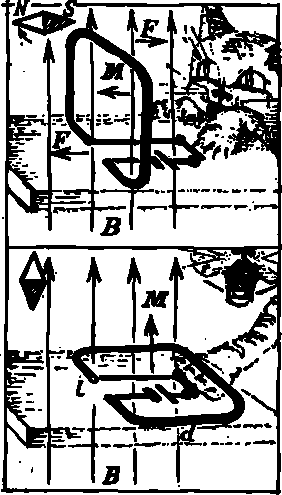
\includegraphics[width=0.4\textwidth]{figures/fig-03-01.pdf}
\caption{A loop of wire in a magnetic field showing the magnetic moment.}
\label{fig-3.1}
\end{figure}

It follows from the foregoing that it would be expedient to introduce a new concept at this point. This concept, as we shall see, proves to be of prime significance. We shall characterize the current loop by the vector $M$, which we shall call the \emph{magnetic moment} (see \figr{fig-3.1}). The magnitude of the magnetic moment is taken equal to the product of the current $I$ by the loop area $A=ld$. Thus
\begin{equation*}%
M=IA
\end{equation*}
Vector $A$ has the direction of the positive normal to the plane of the loop.

Now we have an instrument that can be used to measure a field. It is most convenient to measure the maximum moment of force acting on the test loop.

Going from one point of the field to another or changing the field by moving its sources or varying the currents setting up the field, we obtain different values of the moment of the couple of forces $F$ acting on the test loop. The maximum moment of force can be written as
\begin{equation*}%
N = BM
\end{equation*}
where $B$ is a quantity that we take as the measure of the field. It is called the \emph{magnetic induction}. Thus, the magnetic induction is equal to the maximum moment of force acting on a test loop with unit magnetic moment.

We take the density of lines of force, i.e. their number per unit area, proportional to value $B$. Vector $B$ is directed along the lines of force.


The magnetic moment, magnetic induction and our old friend the moment of force are all vectors. After thinking it over, we must admit that these vectors differ from the vectors of displacement, velocity, acceleration, force, etc. As a matter of fact, the velocity vector, for example, of a body indicates the direction of motion of the body, the vectors of acceleration and force indicate the direction of attraction or repulsion. In these cases, the arrowhead at the end of the line symbolizing the vector has an entirely objective and real meaning. As to our new acquaintances and the moment of force, these are horses of another colour. The vectors are directed along the axis of rotation. It is clear that an arrowhead put at one or the other end of a line symbolizing an axis of rotation is of a wholly arbitrary nature. It is necessary, however, to agree upon the direction of the vectors. An arrowhead at the ``end'' of an axis of rotation is meaningless. But the direction of rotation has an objective meaning, and this is what we should try to specify by the arrowhead. It has been agreed that the arrowhead is put on the axis in such a manner that when we face the arrowhead, rotation is either clockwise or counterclockwise. Physicists are accustomed to the latter.

These two types of vectors have expressive names that speak for themselves: \emph{polar and axial vectors}.

After measuring the fields of various systems, we can formulate the following rules. Magnets always have two poles: a north pole near which each line of force starts and a south pole near which it ends. Naturally, we cannot determine by such experiments what happens to the lines of force inside the magnet.

With respect to the magnetic fields of currents (\figr{fig-3.2}), we discover the following law: the magnetic lines of force are circular and surround the current conductor. If we look along the conductor in the direction of the current, the lines of force have the clockwise direction. A point or an $X$ in diagrams or drawings indicates (and this is universally accepted) that the current flows toward or away from us.
\begin{figure}[!ht]
\centering
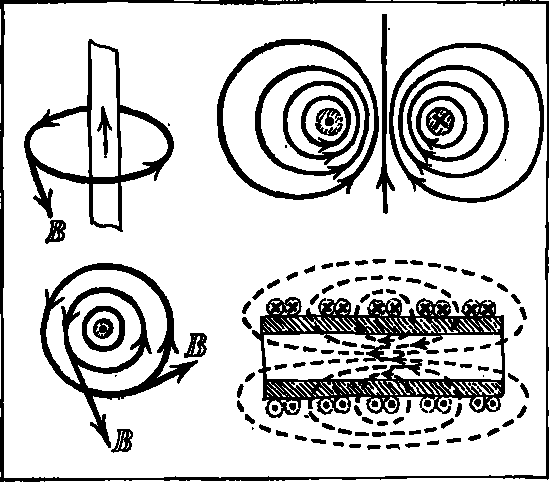
\includegraphics[width=\textwidth]{figures/fig-03-02.pdf}
\caption{Determining the direction of magnetic field from the current.}
\label{fig-3.2}
\end{figure}

As is clear from the formula, the magnetic moment is measured in Amp\`eres multiplied by the loop area in square metres.

The unit of magnetic induction is the \emph{tesla}. One tesla (\si{\tesla}) is equal to \SI{1}{\kilo\gram\per\ampere\second\squared}.

Magnetic fields are set up by currents and permanent magnets. Magnetic fields affect currents and permanent magnets. If for some reason the investigator does not wish to resort to the concept of a magnetic field, he can classify all kinds of interaction in which magnetic fields participate into four groups. These are: magnetic, i.e. the action of a magnet on another magnet; electromagnetic, i.e. the action of a current on a magnet; magnetoelectric, i.e. the action of a magnet on a current; and, finally, electrodynamic, i.e. the action of a current on a current.\label{mag-interaction}

This terminology is mainly used in engineering. An instrument is said to be magnetoelectric, for instance, if the magnet is fixed and the current-carrying loop is movable.

The electrodynamic interaction is the basis for the modern definition of a unit of current. This definition is as follows: an \emph{ampere} is the equivalent of a constant current which, in passing along two parallel and straight conductors of infinite length and negligible cross section, located in a vacuum at a distance of one metre from each other, would develop a force between these conductors equal to \SI{2d-7}{\newton\per\metre} of length.\label{ampere-def}



In the International System of Units (SI), accepted all over the world, the Amp\`ere is one of the fundamental units.\footnote{In a revision of SI Units in 2019, the definition of ampere underwent a major revision. The ampere is now defined by setting the magnitude of the elementary charge to \num{1.602176634d-19} which means an ampere is an electrical current equivalent to \num{d19} elementary charges passing every \num{1.602176634} seconds. -- Damitr} Correspondingly, the coulomb is defined as an \emph{ampere-second}. I must admit to the reader that I prefer the system in which the quantity of electricity is the fundamental unit and is expressed in terms of the mass of deposited silver in electrolysis. But metrologists must know best. Evidently, the above definition must have some merits, though, it seems to me that in practice a measurement of the electrodynamic force with high accuracy is a far from simple matter.

Since he now knows how to determine the direction of a magnetic field, as well as the rules for finding the direction of the force exerted on the current by a magnetic field (to be discussed a little further on), the reader can deduct for himself that currents flowing parallel in the same direction attract one another, and those flowing in opposite directions repel one another.

\section{Effects of Uniform Magnetic Field}
A magnetic field is said to be \emph{uniform} if its effect on any device indicating its presence is the same at various places in the field. Such a field can be set up between the poles of a magnet. Naturally, the closer to each other the poles are located and the larger the flat end faces of the magnet, the more uniform the field.

We have already discussed the effect of a uniform magnetic field on a magnetic needle and on a current loop: if there is no counterbalancing spring, then they locate themselves in the field so that their magnetic moment coincides with the direction of the field. Their ``north pole'' faces the ``south pole'' of the magnet. This fact can be expressed in the words: the magnetic moment becomes aligned with the lines of force of the magnetic field.

Let us consider the effect of a magnetic field on moving charges.

It is utterly simple to show that such an effect exists and that it is no small one. We just take a plain horseshoe magnet of the kind used in school physics classes and bring it near an electron beam produced by an electron gun. The bright spot on the fluorescent screen is displaced and moves from place to place as we move the magnet.

From a qualitative demonstration of this phenomenon we can pass on to a quantitative investigation. We find that the force exerted by a magnetic field of magnetic induction B on an electron travelling at the velocity $v$ at right angles to the lines of force is
\begin{equation*}%
F = e v B
\label{lorentz-force}
\end{equation*}
where $e$ is the charge of the particle (this law is valid, not only for electrons, but for any charged particles). 
\begin{figure}[!ht]
\centering
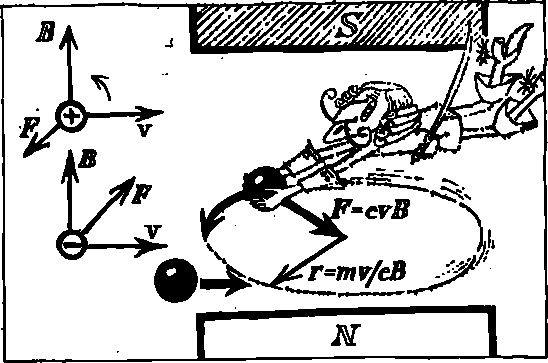
\includegraphics[width=\textwidth]{figures/fig-03-03.pdf}
\caption{The force on a charged particle in a magnetic field.}
\label{fig-3.3}
\end{figure}
When, however, a charged particle travels along a line of force in a magnetic field, the field has no effect on the particle. Readers familiar with trigonometry should have no difficulty in writing an equation for the force exerted on a particle travelling at some angle to the direction of the field. We shall not clutter up the text with equations that will not be required further on. 

But we have not yet said anything about the direction of the exerted force, though this is of prime importance. Experiments show that the force is perpendicular both to the direction of motion of the particle and to the magnetic induction. In other words, the force is perpendicular to a plane passing through vectors $v$ and $B$. But this is not all. Every medal has two sides. How do they differ in our case? In the direction we must rotate one vector so that it coincides with the other. If we see the rotation of vector $v$ toward vector $B$ through the angle less than \ang{180} as being counterclockwise, we are on the side of the positive normal.

The simple vector diagrams at the left in \figr{fig-3.3} indicate that a positively charged particle is deflected by the field in the direction of the positive normal. An electron is deflected in the reverse direction.

Consider now the interesting result that follows from this law for an electron flying at right angles into a constant magnetic field (at the right in \figr{fig-3.3}). Try to figure out the path described by the electron in the field. It will, of course, travel in a circle. The force exerted by the field is a centripetal force and we can readily calculate the radius of the circle by equating $mv^{2}/r$ and $evB$. Thus, the radius of the path is
\begin{equation*}%
r = \frac{mv}{eB}
\end{equation*}
Note that we could calculate the properties of a particle from its behaviour. But again we find ourselves in the same predicament as when we investigated the motion of particles in an electric field. We cannot determine the electric charge and the mass of the particle separately! Here as well we determine the ratio $e/m$.

Thus, a particle travels along a circle if its velocity is directed at right angles to the magnetic field; a particle travels by inertia if its velocity is directed along the magnetic field. What does it do in the general case? Your answer is ready, of course. The particle travels along a helix whose axis is a line of force. The helix consists of tightly or loosely wound coils, depending upon the initial angle of entry of the electron into the magnetic field.

Since a magnetic field acts on a moving particle, it should also exert a force on each piece of wire carrying a current. Consider a portion of length $l$ of an electron beam. Assume that there are n particles in this portion. The force exerted on a wire of the same length, along which the same number of particles travel at the same velocity, is equal to $nevB$. The current is equal to the total charge passing through the wire in unit time. The time $\tau$ during which the electrons being discussed travel a path $l$ equals
\begin{equation*}%
\tau = \frac{l}{v}
\end{equation*}
This means that we can write the equation for the current as
\begin{equation*}%
I  = \frac{ne}{\tau} = \frac{nev}{l} 
\end{equation*}
Substituting the velocity from this equation
\begin{equation*}%
v  = \frac{Il}{ne}
\end{equation*}
into the formula for the force acting on a portion of an electron beam, we obtain the force exerted on a conductor of length $l$, Thus
\begin{equation*}%
F = I l B
\end{equation*}
This is valid only when the wire is perpendicular to the field.

The direction that a wire carrying a current is deflected can be determined by the diagram shown in \figr{fig-3.3}. In deference to the investigators working in the $19^{\textrm{th}}$ century, I have included \figr{fig-3.4}. As a matter of fact, this drawing is not of only pure academic interest. It can serve as an aid in remembering the rule for the deflection of currents in magnetic fields. The drawing shows how the field set up by a current (flowing away from us) combines with the external field. The result of this combination is illustrated at the right. If we conceive of lines of force as being tensioned ether and having material properties (a widespread point of view last century), the direction the conductor is displaced can be visually interpreted: the conductor is simply pushed out by the field.
\begin{figure}[!ht]
\centering
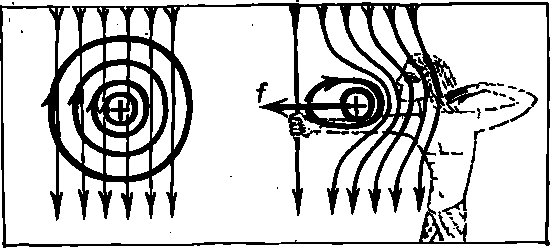
\includegraphics[width=\textwidth]{figures/fig-03-04.pdf}
\caption{Deflection of current in a magnetic field.}
\label{fig-3.4}
\end{figure}
Next we shall demonstrate that the effect of a magnetic field on a moving charge and on a piece of current-carrying conductor is the same phenomenon with which we began our discussion of the effects of a magnetic field.

Let us return to \figr{fig-3.1}. It shows the forces acting on a current-carrying loop. No forces are exerted on the sections of the wire that are aligned with the field. The force couple acts on the other two sections. We can see from the drawing that the moment of this couple is precisely equal to the product of the force by the arm:
\begin{equation*}%
N=IlBd=IAB= MB
\end{equation*}
Thus the expression for the moment of force as the product of the magnetic moment of the loop by the magnetic induction follows directly from the equation for the force exerted on a charge.

The formula $F=evB$ with which we began this section is called the \emph{Lorentz equation} after Hendrik Antoon Lorentz (1853-1928), the Dutch physicist who proposed it in 1895.

\section{Effects of Nonuniform Magnetic Field}

It is quite easy to set up a nonuniform magnetic field. We can, for instance, impart curved shapes to the faces of the poles as shown in \figr{fig-3.5}. Then the paths of the lines of force are as illustrated.

\begin{figure}[!ht]
\centering
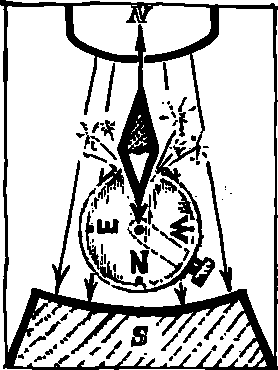
\includegraphics[width=0.4\textwidth]{figures/fig-03-05.pdf}
\caption{Lines of force in a non-uniform magnetic field.}
\label{fig-3.5}
\end{figure}

Assume that the poles are sufficiently far away from each other and place a magnetic needle near one of the poles. As mentioned before, such a needle can move in a straight line, in the general case, as well as rotate. We observe rotary motion alone of a needle or current loop only if the magnetic field is uniform. Both kinds of motion occur in a nonuniform field. The needle turns so that it is aligned with the lines of force and is attracted toward a pole (see \figr{fig-3.5}). It is pulled into the region where the field is stronger. (The artist has, of course, overdone it; it is improbable that even an extremely strong field can split the compass in two.)

To what is this behaviour due? Evidently, to the fact that not only a force couple acts on the needle in a non-uniform field. The ``forces'' exerted on the north and south poles of a needle placed in a nonuniform field are not the same. The end located in a stronger region of the field is subject to a larger force. Therefore, after the needle turns, the arrangement of the forces is as shown in the drawing. There is an excess force exerted toward the side where the field is stronger.

True, a current loop of exceptionally thin wire behaves in exactly the same way. Thus, in beginning with a model of a needle with two ``poles'', my aim was only to provide a more pictorial representation.

What, then, is the law of nature pertaining to our phenomena? What is the force equal to? Experiments and calculations indicate that, for any system having the magnetic moment $M$, this force is the product of the moment of the system by the slope of the curve representing the increase in the field strength (magnetic induction).

Assume that the magnetic needle aligns itself with a line of force. The magnetic induction values differ at the places where the north and south poles of the magnetic needle are located. We plot a curve of the field along the line passing through the poles. For the sake of simplicity, we replace the section of the true field curve between the poles with a straight line. The shorter the needle, i.e. the closer its poles to each other, the more accurate our approximation. The slope of the curve, i.e. the tangent of the angle our straight line on the diagram makes with the horizontal axis, is equal to the quotient of the difference in the values of the field strength divided by the length of the needle. Thus
\begin{equation*}%
F = M \frac{(B_{N}-B_{S})}{l}
\label{force-mag}
\end{equation*}
where $l =$ length of the needle; and $B_{N}$ and $B_{S}=$  field strengths at the north and south ends of the needle. (Do not be surprised that the tangent of an angle turns out to be a dimensional quantity.)

If we replace the fraction by the value of the tangent of the angle of inclination of the straight line tangent to the curve representing the field at the point where the particle interesting us is located, the ``poles disappear'' and the formula is valid for any particle or system of particles.

In conclusion, we can say that in a nonuniform field a system or a particle with a magnetic moment is attracted to the poles of the magnet or repelled by them in accordance with the direction of the magnetic moment: either along with or opposite to the lines of force.

But can the magnetic moment align itself against the direction of the field? It certainly can! We shall discuss below the cases in which this occurs.

\section{Amp\`erian Currents}

Right up to the nineteenth century it was no difficult matter to advance a physical theory. If a body becomes heated, that means it contains more caloric. If a medicine makes you fall asleep sooner, it contains a soporific power. Certain rods, made of iron ores, point to the north. A strange behaviour, but immediately understood if we say that such rods and needles possess a magnetic spirit. We know that magnetic needles have rendered good service to seafarers since ancient times. But sometimes they played tricks. So what; no problem: evil spirits are to blame! Likewise, it was no surprise that iron, steel and certain alloys could be magnetized. These are simply bodies that a magnetic spirit (or soul) can easily be imparted to.

After the discoveries made by Oersted and Amp\`ere, it became clear that a bridge could be constructed between electrical and magnetic phenomena. At one time, two theories enjoyed equally wide support. From one point of view, everything became clear if we assume that the wire along which an electric fluid flows is converted into a magnet. The other point of view was expounded by Amp\`ere. He contended that the magnetic spirit of iron ores consists of microscopic electric currents.

Amp\`ere's point of view seemed to be more logical. No particular importance was attached to this theory because, in the first half of the nineteenth century, no one even dreamt of the feasibility of really discovering such currents. They even doubted that the world is built up of atoms and molecules.

But in the twentieth century, when physicists conducted a whole series of ingenious experiments that proved that the world around us consists of atoms and that atoms consist of electrons and atomic nuclei, the existence of Amp\`erian currents was finally taken to be a real fact that could be employed in an effort to understand the magnetic properties of substances. Most scientists agreed that the ``molecular currents'' proposed by Amp\`ere are formed by the motion of electrons about atomic nuclei.

It seemed possible to explain magnetic phenomena by means of these conceptions. As a matter of fact, an electron travelling around a nucleus can be likened to an electric current; we have the right to ascribe a magnetic moment to this system and relate it to the angular momentum of the moving charged particle.


It is extremely simple to prove this last statement.

Assume that an electron revolves in a circle of radius $r$. Since the current equals the charge carried in unit time, the revolving electron can be likened to a current $I=Ne$, where $N$ is the number of revolutions per second. The velocity of the particle can be related to the number of revolutions per second by the equation $v=N \times 2 \pi r$. Then the current equals
\begin{equation*}%
I = \frac{ve}{2 \pi r}
\end{equation*}
It is natural to call the magnetic moment of an electron revolving about a nucleus its \emph{orbital moment}. It equals
\begin{equation*}%
M = IA = \frac{ve}{2 \pi r} \pi r^{2} = \frac{1}{2} evr
\end{equation*}
We remind the reader (see Book~1) that the angular momentum of a particle is $L=mvr$ and find that between the angular momentum and the magnetic moment we have the following relationship that is of great significance in atomic physics:
\begin{equation*}%
M = \frac{e}{2m} L
\end{equation*}
It follows that atoms must have magnetic moments.

By various procedures, on which we shall not dwell here, we can obtain the atomic gas of various substances. Using two slits in a gas chamber we can produce beams of neutral atoms of hydrogen, lithium, beryllium, etc. They can be passed through a nonuniform magnetic field and traces of the beam can be observed on a screen. The question we put to nature is the following: Will the stream of atoms be deflected from a straight line, and if so, how?

The atom has an orbital moment and, consequently, behaves similar to a magnetic needle. If the magnetic moment is directed along the field, the atom is deflected toward the region of a strong field. In antiparallel arrangement of the moment and field, the atom is deflected toward the region of a weak field. The amount of deflection can be calculated by a formula similar to the one given on page \pageref{force-mag} for the force acting on a magnetic needle.

The first thing that occurs to us is that the magnetic moments of atoms are arranged at random. If this is so, we should expect that the trace of the beam is blurred. But experiments yielded entirely different results. The beam of atoms is never blurred; it splits into two, three, four or more components, depending upon the kind of atoms. This splitting is always symmetrical. Sometimes the components of the beam include an undeflected beam, sometimes there is no undeflected beam, and sometimes the beam does not split up at all.

It follows from this experiment, one of the most important ever conducted in physics, firstly, that the motion of electrons about an atom can really be likened to a closed-circuit electric current. It can be likened in a narrow and quite definite sense: like closed-circuit currents, atoms can be ascribed a magnetic moment. Further, the magnetic moments of the atoms can make only certain discrete angles with the direction of the magnetic induction vector. In other words, the projections of the magnetic moments on this direction are quantized.

A great triumph for theoretical physics was the fact that these results had been predicted in elaborate detail. It follows from theory that the angular momentum and the magnetic moment of the electron, due to the motion of atomic electrons in the field of the nucleus (these moments are said to be orbital\footnote{This name is of historical origin: the development of atomic theory began with the supposition that an atom resembles the solar system.}), are antiparallel and their projections on the direction of the field can be written fn the form
\begin{equation*}%
L_{z} = m \frac{h}{2\pi} \qqtext{and} M_{z} = m \mu_{B}
\end{equation*}
where $m=a$ whole number that can take the values 0, 1, 2, 3, \ldots{}; $h/2\pi=$ the smallest value of the projection of the angular momentum; and $\mu_{B}=$the smallest value of the projection of the magnetic moment. The values of $h$ and $\mu_{B}$ are determined from experiments:
\begin{align*}%
h & = \SI{6.62d-27}{(\erg-\second)}, \qand \\
\mu_{B} & = \SI{0.93d-20}{\erg\per\gauss\per\second}
%\label{ang-mom}
\end{align*}
%\TODO 
%\hlred{TODO! check the units of $\mu_{B}$}

We may add that these important constants of physics have been named after the great scientists that laid the foundations of quantum physics: $h$ is called \emph{Planck's constant} after the German physicist Max Karl Ernst Ludwig Planck (1858-1947) and $\mu_{B}$ is the Bohr magneton after the Danish physicist Niels Henrik David Bohr (1885-1962).\label{ang-mom}

The postulates of quantum mechanics were not sufficient, however, to provide a comprehensive understanding of the different ways that the beams of various atoms are split. Even the simplest of atoms, those of hydrogen, behaved unexpectedly. It became necessary to add another exceptionally vital hypothesis to the laws of quantum mechanics. We have already mentioned it once. It consists in ascribing its own (intrinsic) angular momentum, called spin, and the corresponding intrinsic magnetic moment to the electron (or to any elementary particle, as was found later). To understand why it is inevitable to liken the electron to a magnetic needle, we must first investigate in more detail the motion of atomic electrons.

\section{Electron Cloud of the Atom}

It is impossible to observe the motion of an electron. And what is more, we cannot even hope that the advance of science can ever provide the opportunity of seeing an electron. The reason is sufficiently clear. To ``see'' something, we must first ``illuminate'' it. But ``illumination'' means to subject the electron to the energy of some kind of ray. The electron is of such tiny mass that any interference, by means of an instrument for observing it, inevitably causes the electron to leave the place it was previously located at.

Not only the meagre information about the structure of the atom which we are about to convey to the reader, but the whole consistent doctrine of the electronic structure of matter, is the result of theoretical rather than experimental investigations. We are, however, sure of its validity because of the innumerable amount of effects observed in experiments and rigorously derived from theory by logical reasoning. We establish the picture of electronic structure, invisible to us, with the same degree of assurance that Sherlock Holmes established the picture of a crime from the clues left by the criminal.

Primarily, a vast source of confidence in this theory is the fact that the picture of electronic structure is predicted by means of laws of quantum mechanics that were established by other experiments.

We have already mentioned that the atomic number of a chemical element in Mendeleev's periodic table is none other than the charge of its nucleus or, what is the same thing, the number of electrons belonging to a neutral atom. An atom of hydrogen has one electron, an atom of helium has two, lithium has three, beryllium has four, etc.

How do all these electrons travel? This question is far from simple and its answer is of an approximate nature. 

Difficulties arise from the fact that the electrons interact with one another and not only with the nucleus. Fortunately, the mutual repulsion (avoidance) of the electrons plays a smaller role than the motion that is due to the interaction of the electron with the nucleus. Only this circumstance enables us to draw conclusions on the nature of motion of electrons in various atoms.

Nature has allocated to each electron a spatial region in which it travels. According to their shape these regions of the electrons are divided into categories denoted by the letters $s,\, p, \,d,$ and $f$.

The simplest is the ``apartment'' of the $s$-electrons. It is a spherical layer. We know from theory that most of the time the electron is within the spherical layer. Hence, any talk about a circular orbit of such an electron is a crude simplification.

The region of space through which the $p$-electron travels is entirely different. It resembles a dumbbell used for physical exercise. Other categories of electrons have even more complex regions of existence.\label{cloud-shape}

Electronic theory can indicate (though not without resorting to experimental data) how many electrons of each kind each element of Mendeleev's table contains.

Is this distribution of electrons according to their types of motion related to their distribution among the $K,\, L,\, M, \ldots$ energy levels discussed in the preceding chapter? It is, and most directly. Theory and experiments show that electrons belonging to the $K$-level can only be of the $s$-type; to the $L$-level, of only the $s$- and $p$-types; to the $M$-level, of the $s$-, $p$-, and $d$-types; etc.

We shall not discuss the electronic structure of atoms in any particular detail, restricting ourself to an account of the structure of the first five elements of the table. Atoms of hydrogen, helium, lithium and beryllium have only $s$-type electrons. The boron atom has four $s$-electrons and one $p$-electron.


The spherical symmetry of the region of space in which the $s$-electron travels casts a doubt on our discussion of the magnetic moment of an atom containing a single electron. As a matter of fact, since the angular momentum can take on identical values directed to all sides with equal probability, the average rotational moment and, consequently, the magnetic moment of such a system should equal zero. Quantum physics also reaches this same natural conclusion: atoms containing only $s$-electrons cannot have a magnetic moment.

But if this is so, the beams of atoms of the first four elements of Mendeleev's table should not be deflected in a nonuniform magnetic field. Is this what we observe? It was found that these predictions are upset for the atoms of hydrogen and lithium. Beams of these atoms behave in an exceptionally strange manner. In both, the beam of atoms is split into two components deflected in opposite directions the same distance from the initial direction. Incomprehensible!

\section{Magnetic Moments of Particles}

Electron spin made its first appearance on the scene in 1925. The necessity of including it in the participants of the events taking place in the microcosm was first revealed by Samuel Abraham Goudsmit (1902-1978) and George Eugene Uhlenbeck (1900-1974). Proposing that the electron has its own (intrinsic) angular momentum, these two investigators showed that all the confusion that had accumulated by that time in the interpretation of atomic spectra could be readily eliminated by this new concept.

The experiments mentioned above for splitting atomic beams were performed somewhat later. When it became clear that here also only the concept of spin could provide a complete explanation of the observed facts, all physicists finally accepted it.

A short time elapsed and it was found that intrinsic angular momentum, or spin, is a property possessed by all elementary particles and not only electrons.

We have already mentioned that the name spin is witness to a natural tendency toward visualization. Since the angular momentum was first introduced in physics as a property of a rotating solid, certain physicists immediately resorted to the graphic picture of a particle rotating about its axis when it was found necessary to ascribe a certain value of the angular momentum to elementary particles in order to save the conservation laws. This na\"ive concept holds no water: we have no more right to speak of an elementary particle rotating about its axis than we would of a mathematical point.

The supporters of visualizability were able to assess the size of the electron on the basis of certain circumstantial evidence. To be more exact, they established that if this concept is applicable to the electron, its size must be less than a certain definite value. The value of spin is known; we shall give it on the following page. Assuming a shape for the electron, we can calculate with what velocity ``points on its surface'' rotate. This velocity was found to be greater than that of light. Thus, if we are persistent in advocating such particle rotation, we must throw overboard the theory of relativity.


Perhaps, the most irrefutable argument against visualizability is the fact that the neutron, which carries no electric charge, possesses spin. Why is this argument decisive? Judge for yourself.

If a particle can be conceived of in the form of a charged sphere, its rotation about its axis should produce something resembling an Amp\`erian current. But if a neutral particle also has angular momentum as well as a magnetic moment (we shall mention these properties of the neutron briefly in Book~4), any analogy with an Amp\`erian current is out of the question.

It does not pay, of course, to pose as a prophet and state that spin and magnetic moment of elementary particles will never be made clear, even on the basis of some more general, as yet undiscovered, law. This problem has been partly solved by the theory of the brilliant English physicist Paul Adrien Maurice Dirac (1902-1984). But we cannot give our reader even a general idea of this theory; it is so abstract. But, as for today, we must consider the ``arrows'' representing the angular momentum and magnetic moment of a particle to be primary concepts (not reducible to something simpler).

About fifty years ago, the majority of physicists upheld the point of view of Einstein, who wrote: ``Every physical theory should be such that it can be illustrated, apart from any calculations, by means of simple images.'' Alas, this opinion of the great thinker turned out to be mistaken. For many years, physicists have been calmly applying theories containing measurable quantities that we cannot associate with any visual image.

The electron and other elementary particles have no ``poles''. In many cases, we confidently speak of them as point particles, agreeing that the idea of shape is not applicable to elementary particles. Nevertheless, we are obliged to ascribe to them two vector properties, an angular momentum (spin) and a magnetic moment. These two vectors always lie along a single line and are parallel in some cases and antiparallel in others.

Experiments show that the general formulas for the projections of the angular momentum and the magnetic moment, given on page~\pageref{ang-mom}, are also valid for the intrinsic moments as well. All experiments, both in spectral analysis and in splitting atomic beams in a nonuniform magnetic field, can be irreproachably interpreted if quantity $m$ in the formula for the projection of the angular momentum of an electron is allowed to take two values: $\pm 1/2$. As for the formula for the projection of the magnetic moment, quantity $m$ can also have two values: $\pm 1$.

Electron spin has the numerical value $(1/2) (h/2\pi)$ and may be disposed only in two directions: along the field or against the field. As to the magnetic moment of the electron, it imitates the spin, also having only two orientations in the field. Its numerical value equals one Bohr magneton.

Now let us return to the experiments with atomic beams. We shall show how easily all the specific features of atomic beam splitting can be explained by the concept of spin.

Indeed, how can we explain the fact that beams of helium and beryllium atoms do not split? As follows. The electrons of these atoms have no orbital moment because they are of the $s$ ``kind''. As to the spins of the electrons, they are in opposite directions. As a matter of fact, this statement does not follow from anything,
though intuitively seems quite natural. The principle, according to which a pair of electrons in an atom establish themselves so that their spins are opposed, is called Pauli's exclusion principle, after the Austrian-Swiss physicist Wolfgang Pauli (1900-1958).

So many hypotheses! Yes, quite a few. But taken all together they form the shapely structure of quantum physics from which so many consequences follow that there is not the least uncertainty but that spin must be ascribed to the electron, that the value of 1/2 must be given to the spin quantum number and that the spins
of a pair of electrons must obey the Pauli principle. Not even a single physicist has a shadow of a doubt on these matters. The sum of these hypotheses represents the structure of the microcosm.

Let us return to our atomic beams. We have just explained why no splitting is observed in beams of helium and beryllium atoms.

But why do hydrogen and lithium behave differently? The hydrogen atom has a single electron. Its orbital moment equals zero because it is an $s$-electron. The projection of its spin can have only two values: plus 1/2 and minus 1/2, i.e., the spin can be aligned either opposite to or along the direction of the magnetic field. This is why an atomic beam splits into two components. The same occurs with lithium atoms because two of its electrons ``compensate for'' their spin and the third behaves like the single electron of the hydrogen atom.

The atoms of other elements that have a single unpaired electron in their outer shell behave in exactly the same way.

To explain why the atomic beams of other elements split into a large number of components it would be necessary to cite several other theorems without giving their proof. They are proved in quantum physics. By taking into account the facts that only $s$-electrons have no orbital moment and that the spin of an electron is manifested only when the electron is alone at its energy level, physicists managed to comprehensively explain the behaviour of atomic beams of all kinds. After studying this fascinating chapter of physics even the staunchest skeptic becomes convinced that all the unproved assumptions accepted in quantum physics are general
laws of nature.

I fear that many readers may remain unsatisfied by these statements. Experiments on the deviation of atomic beams in a nonuniform magnetic field are insufficient in themselves, of course, to introduce such a strange concept as spin. This book is too small, however, for me to cite the vast number of facts that demand full rights for spin among the authentic phenomena of the physical sciences.

For example, how worthy as such proof is the phenomenon of magnetic resonances, having nothing in common with the aforesaid. Radio waves of the centimetre range are absorbed by a substance if they have to flip (invert) the spin. No difficulty is encountered in calculating the energy of the interaction between the magnetic moment of an electron and the constant magnetic field into which the substance is placed in magnetic resonance experiments. This energy constitutes the difference between two energies (parallel and antiparallel arrangement), which is equal to a quantum of the absorbed electromagnetic wave. We can determine the value of the wave frequency in this experiment with exceptionally high precision, verifying the fact that it absolutely coincides with the frequency we calculated on the basis of the known induction of the field and the value of the electron's magnetic moment.

This phenomenon forms the foundation for a large branch of science: the study of electron resonance. It is remarkable that the same events, but, naturally, in another wavelength range, are observed for atomic nuclei. Nuclear magnetic resonance is the most essential method used in studying the chemical structure of substances.

Before going on, it will, perhaps, be helpful to sum up all the facts concerning systems that set up magnetic fields and respond to the presence of a magnetic field.

First of all, we must emphasize again that Amp\`ere's hypothesis was only partly substantiated: magnetic fields are set up not only by moving electric charges. Other sources of magnetic fields are elementary particles, primarily electrons, which have an intrinsic magnetic moment. The technical classification of the kinds of interaction, given on page~\pageref{mag-interaction}, turns out to be inexact. Magnetic fields are set up, by natural and artificial magnets, by electric currents (including streams of electrical particles in a vacuum), as well as elementary particles. The same systems, as well as the particles, respond to the action of magnetic fields.

\begin{figure}[!ht]
\centering
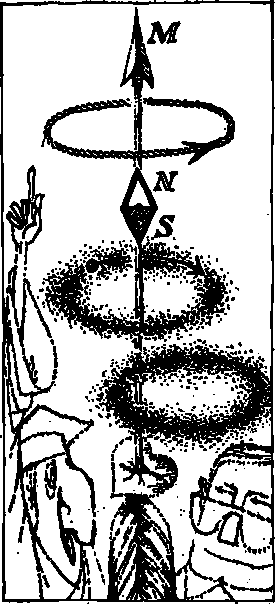
\includegraphics[width=0.4\textwidth]{figures/fig-03-06.pdf}
\caption{The intrinsic magnetic moment of elementary particles characterises  microscopic and macroscopic phenomena.}
\label{fig-3.6}
\end{figure}

The main quantity characterizing a magnetic field and its effects is the magnetic moment vector. For currents, this vector depends upon the shape of the current loop. The moment of a needle is related in a complex manner to the atomic structure of the substance, but it can be readily measured. Electrons travelling in the field of the nucleus have an ``orbital'' magnetic moment as if (note, please, this ``as if'') their motion about the nucleus generated an electric current. Finally, the intrinsic magnetic moment is a primary property that characterizes elementary particles.

\figr{fig-3.6} should help you to remember this fundamental information. This drawing represents the sum of our knowledge today about the ``magnetic soul'' or, if you please, the magnetic heart. The French for a magnet is ``aimant'' (from the verb ``aimer'' -- to love). The drawing underlines the fact that macroscopic current, a bar magnet, the orbital motion of the electron and the electron itself are all characterized by a single physical concept.


\section{Electromagnetic Induction}
Experiments show that a beam of electrons travelling in a magnetic field is deflected from a straight line. As mentioned on page~\pageref{lorentz-force}, the force responsible for this deflection, called the Lorentz force, is directed perpendicular to the magnetic lines of force and to the velocity vector of the electrons. It is determined by the formula $F = evB$. This is the simplest expression for the Lorentz force and is valid when the direction of the electron velocity makes a right angle with the direction of the magnetic field.

If to this fact we add our certainty that a metal conductor contains free electrons, we can, by simple reasoning, come to the conclusion that upon certain motions of a conductor in a magnetic field an electric current should be produced in the conductor.

\begin{figure}[!ht]
\centering
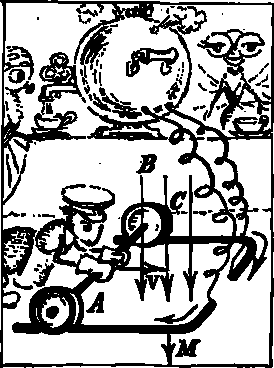
\includegraphics[width=0.4\textwidth]{figures/fig-03-07.pdf}
\caption{The electromagnetic induction is observed when there is a motion of a conductor in a magnetic field.}
\label{fig-3.7}
\end{figure}


This phenomenon, which, we might say, is fundamental for all modern engineering, is called \emph{electromagnetic induction}. We shall proceed to derive its formula.

Illustrated in \figr{fig-3.7} is a current-conducting loop consisting of rod $AC$ of length $l$, which rolls along metal wires between the poles of a magnet without breaking the circuit of the loop. If the rod is rolled in the direction perpendicular to the lines of force, its electrons are subject to a force and an electric current flows along the loop circuit.

We reach a conclusion whose importance cannot be overestimated: an electric current can be produced in a conductor of a closed circuit even if the circuit contains no storage battery or other current source.

We can calculate the emf, i.e. the work required to carry unit charge along the closed loop. Work is the product of a force by the path. It is performed only on the part of the loop moving in the field. The length of the path is $l$ and the force per unit charge is $vB$.

This developed electromotive force is called the induced emf. Its value is determined by the formula
\begin{equation*}%
\mathcal{E}^{\textrm{ind}} = vBl
\end{equation*}
It is desirable to generalize this formula so that it is suitable for any motion of any conducting loops. We derive this generalization as follows. During time $\tau$ the rod-type conductor travels the distance $x$, its velocity $v$ being equal to $x/\tau$. The area of the conducting loop is reduced by the amount $A = xl$. Then the formula for the induced emf takes the form
\begin{equation*}%
\mathcal{E}^{\textrm{ind}} = \frac{BA}{\tau}
\end{equation*}
What does the numerator in this formula signify? This is sufficiently clear: $BA$ is the amount of change in the magnetic flux (the number of lines of force) through the loop.

Our proof has, of course, been carried out for a very simple case. The reader will have to take my word that an entirely rigorous proof can be carried out for any case. The formula obtained is of most general application and the law of electromagnetic induction can be formulated as follows: an induced emf is always developed when the number of lines of force through the loop is changed. Here the value of induced emf is numerically equal to the change of magnetic flux per unit time.

There may be movements of a loop in a magnetic field that induce no current. There is no current when the loop moves in a uniform field parallel to the lines
of force. If the loop is rotated in a uniform magnetic field, a current is induced. This also occurs when the loop is moved away from or toward a pole of a bar magnet.

Experiments indicate that our generalization is even more significant than we have found so far. We considered cases in which the current loop and the source of the magnetic field changed their relative positions. The last formula we derived says nothing about any motion. The only factor is the change of magnetic flux. But a change in the magnetic flux through a conducting loop does not necessarily involve a mechanical displacement.

\begin{figure}[!ht]
\centering
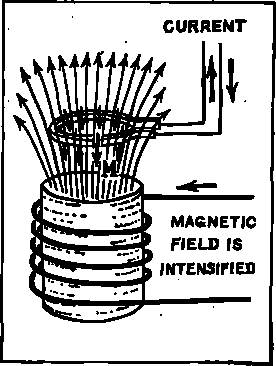
\includegraphics[width=0.4\textwidth]{figures/fig-03-08.pdf}
\caption{A varying current also changes magnetic flux resulting in electromagnetic induction.}
\label{fig-3.8}
\end{figure}

As a matter of fact, we can use, as the source of the magnetic field, not a permanent magnet, but a loop or, even better, a coil through which a current from any outside source is passed. By means of a rheostat or in some other way we can vary the current in this primary coil which is the source of the magnetic field. Then the magnetic flux through the loop changes even though the source of the magnetic field and the conducting loop are stationary (\figr{fig-3.8}).


Will our generalization be valid in this case as well? This question can be answered by an experiment, and the answer is ``yes''. Regardless of how the number of lines of force is changed, the formula for the induced emf, given on the preceding page, is valid.


\section{Direction of Induced Current}

Next we shall demonstrate that a simple universal rule exists for the direction of induced currents. Let us consider several examples from which we shall draw a general conclusion.

Returning to \figr{fig-3.7} we can note the following. When we reduce the area of the loop, the magnetic flux through the loop is reduced. The direction of the current shown in the drawing is such that the magnetic moment of this induced current is directed along the lines of force. This means that the intrinsic field of the induced current is directed so as to ``hinder'' the reduction of the magnetic field. We reach the same conclusion in the reverse case. When the area of the loop is increased, the flux through the loop is also increased. But now the magnetic moment or the loop is directed against the lines of force. Again we find that the field of the induced current hinders the action that causes it.

\begin{figure}[!ht]
\centering
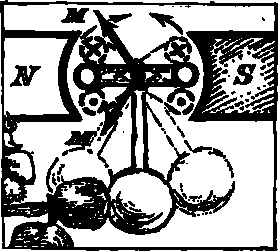
\includegraphics[width=0.4\textwidth]{figures/fig-03-09.pdf}
\caption{Finding the direction of the induced current.}
\label{fig-3.9}
\end{figure}


Another example. Assume that the loop is located between the poles of the magnet in such a manner that the flux through it is equal to zero. Then we begin to turn the loop clockwise and counterclockwise. Both cases are illustrated in \figr{fig-3.9}. Solid lines show the projection of the loop in the initial position; dash lines show the projections in the turned positions when the current is induced. Using the left-hand rule, we find the direction of the induced current in each case. In our drawing, the north pole is shown at the left. Consequently, when the loop is turned clockwise, the magnetic moment of the induced current faces downward; when the loop is turned counterclockwise, it faces upward. As the angle of rotation is increased, the intrinsic magnetic field of the loop (in either case) reduces the field causing the induction more and more. Again the same rule is valid.


Next we shall see how our loop behaves in nonuniform fields. Return to \figr{fig-3.8}. Assume that the current of the electromagnet is constant. What happens when we displace the loop? When we move the loop toward the north pole, the magnetic moment is directed against the lines of force. If the loop is moved away from the pole, the intrinsic field of the induced current strengthens the field. We can predict such behaviour by again resorting to the left-hand rule.

How about magnetic fields set up by alternating currents? Any increase or decrease of the current in the primary coil leads to a change in flux. An emf is induced in the loop (see \figr{fig-3.8} again).

How can we determine the direction of the current? We can no longer use a hand rule because there is no motion. This is where our generalization comes in handy.
It was found that in this case as well the direction of the current, induced by reducing or increasing the number of lines of force through the loop, obeys the same rule: the induced current sets up a field in the direction that compensates for the change in the magnetic field causing the induction.

%\newpage

\begin{center}
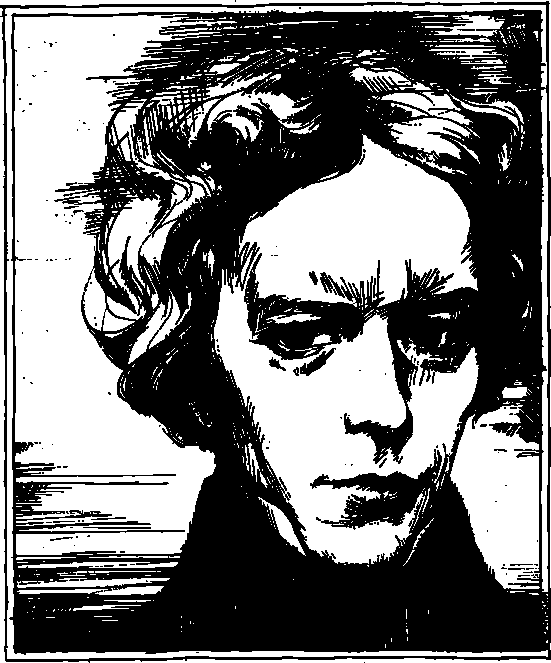
\includegraphics[width=0.8\textwidth]{figures/faraday.pdf}
\end{center}
{\small \textsf{{Michael Faraday [1791-1867]} -- \textsf{\footnotesize famous English physicist; he discovered electromagnetic induction (in 1831). This was no chance discovery; Faraday searched for it. Faraday's laws of electromagnetic induction are the foundation of electrical engineering. It is difficult to overestimate the importance of the laws of electrolysis established by Faraday. This great scientist introduced and explained such terms, so widely used today, as anode, cathode, anion, cation, ion and electrolyte. Faraday proved that the intermediate medium influences electrical interaction. Mention must be made of the discovery of magnetic rotation of the plane of polarization. The fact that all bodies belong either to paramagnetic or to diamagnetic materials was also established by Faraday. The world had never known a more gifted experimental physicist than Michael Faraday.}}}




\section[Discovery of the Law of EMI]{Discovery of the Law \\of Electromagnetic Induction}
\normalfont

The discovery of electromagnetic induction belongs to those rare events that have a decisive influence on the progress of mankind. It would therefore be unpardonable not to dwell to some extent on the history of this discovery. It was made a long time before the investigation of the behaviour of an electron beam in a
magnetic field. The historical course of events does not coincide in any way with the sequence we chose in the preceding sections for expounding this subject. Logic and the continuity of thought from item to item are not at all obliged to proceed in parallel with the historical succession of events.

Up to the time when Michael Faraday began his experiments that led to the discovery of electromagnetic induction, the situation in the science of electric and magnetic fields was the following.

By this time, the production of a direct current and the laws of its behaviour in electric circuits posed no serious problems to physicists. The effects of current
on a permanent magnet and the interaction of currents had been established. It became clear that a direct current sets up a magnetic field surrounding the conductor. This field can be measured either with a magnet or by means of another current. This raised the question of the inverse phenomenon: Can a magnetic field produce a current in a conductor?

In an entry made in 1821 in his diary, Faraday set himself the task of converting magnetism into electricity. It took this great scientist ten years to achieve this aim. He had failed for so many years because he tried to obtain a current by placing a conductor in a constant field. But in 1831, his persistent efforts finally succeeded. The quotation given below, from an article written by Faraday in 1831, is the first description of this phenomenon.

\begin{quote}
``\textbf{10.} { Two hundred and three feet of copper wire in one length were coiled around a large block of wood; other two hundred and three feet of similar wire were interposed as a spiral between the turns of the first coil, and metallic contact everywhere prevented by twine. One of these helices was connected with a galvanometer, and the other with a battery of one hundred pairs of plates four inches square, with double coppers and well charged. When the contact was made, there was a sudden and very slight effect at the galvanometer, and there was also a similar effect when the contact with the battery was broken. But whilst the voltaic current was continuing to pass through one helix, no galvanometric appearances nor any effect like induction upon the other helix could be perceived, although the active power of the battery was proved to be great, by its heating the whole of its helix and by the brilliancy of the discharge when made through charcoal.}''
\end{quote}

The discovery of electromagnetic induction was the first stage in the next twenty years of Faraday's investigations whose aim was to find a unified relationship between all electrical and magnetic phenomena.

In discussing electromagnetic induction, we should also mention the names of other prominent physicists. The American physicist Joseph Henry (1797-1878) discovered self-induction in 1832. If the current in a coil changes, the magnetic field set up by this current also changes, thereby changing the flux of the field passing through this same coil and inducing an emf in its ``own'' circuit.

And who discovered the law governing the direction of the induced emf? The most comprehensive answer to this question can be found in the works of Lenz. Lenz's law determines the direction of the induced current. ``If a metal conductor is moved near a current or magnet, a galvanic current is induced in the conductor. The direction of this current is such that if the wire were at rest, it would begin to move in the direction directly opposite to the actual movement. It is assumed that the wire can move both in the direction of its actual motion and in the opposite direction.''

After 1840, a unified concept of electromagnetism was developed, step by step. The discovery of electromagnetic waves was the last and, evidently, most brilliant step.


\section{Induced Eddy Currents}
If currents can be induced in wire conductors, it would seem quite natural that they can also be induced in heavy solid pieces of metal. Each piece of metal contains free electrons. If the metal moves in a constant magnetic field, the free electrons are subject to the Lorentz force. The electrons describe circular paths, i.e, form eddy currents. This phenomenon was first observed in 1855 by the French physicist Jean Bernard L\'eon Foucault (1819-1868).

The laws of electromagnetic induction are equally valid whether the magnetic flux changes due to relative displacement of the metal and the source of the field or whether the magnetic field changes due to motion of the electric current setting up the field. Consequently, eddy currents are induced when the magnetic field changes with time and not only when there is a relative motion. The most convincing experiment illustrating the latter is dropping a coin between the poles of a strong
magnet. It drops as if in viscous oil rather than with the usual acceleration. The idea of this experiment is obvious: eddy currents are induced in the coin. Their direction, according to Lenz's law, is such that their interaction with the primary magnetic field brakes the motion that causes the induction.

Among the useful applications of eddy currents are the following. In the first place, they are used in the so-called induction furnaces for heating to high temperatures and even melting metals. Secondly, they provide for ``magnetic damping'' in many indicating instruments.

An ingenious invention (and this is thirdly) is the electric meter. You have, of course, noticed that its main component is a rotating disk. The more lights you turn on or electric appliances you plug in, the faster the disk rotates.

The principle of this device consists in having two currents. One is in a circuit parallel to the load and the other is the load current itself. These currents flow in coils wound on iron cores. The alternating current magnetizes the iron cores. Since we have an alternating current, the poles of the electromagnets are continually being reversed. A sort of running magnetic field is set up between their poles. The coils are arranged so that the running field formed by both coils induces eddy currents in the body of the disk. The direction of these eddy currents is such that the running magnetic field pulls at the disk, rotating it.

The speed of rotation depends upon the currents in both coils. As can be shown by exact calculations, this speed is proportional to the product of the current by the voltage and by the power factor (cosine of the phase angle) or, in other words, to the consumed power. We shall not dwell on the simple mechanical transmission connecting the rotating disk to the counter for indicating the watt-hours of energy used.

In the majority of cases, however, efforts are made to eliminate eddy currents. This is one of the concerns of designers of electric machinery. As all other currents,
eddy currents utilize some energy of the system. These energy losses may reach such high values that it becomes necessary to resort to all kinds of contrivances. The simplest method of combatting eddy current losses is to replace large solid pieces of metal in electric machines with laminated sheet stock. In sheet metal, the eddy currents lack sufficient ``elbowroom'', their magnitudes are substantially lower and we obtain a corresponding drop in heat losses.

The reader has undoubtedly noticed that transformers become heated. At least one-half of the heating is due to the effect of eddy currents.

\section{Inductive Surge}

Highly perfected methods of measuring magnetic fields can be devised by making use of electromagnetic induction. Thus far we proposed using a magnetic needle for this purpose, or a test loop with a known direct current. The magnetic induction was determined by the magnitude of the moment of force acting on the test loop or needle whose magnetic moment is equal to unity.

Now we proceed in a different manner. After connecting a tiny current loop to a measuring instrument, we locate it perpendicular to the lines of force and then, with a rapid motion, turn the loop \ang{90}. As the loop is turned, a current is induced in it and a quite definite quantity $Q$ of electricity, which can be measured, flows through the loop circuit. In what way is this quantity of electricity related to the strength of the field at the point where we located the test loop?

The necessary calculations are sufficiently simple. According to Ohm's law, the current $I$ is the quotient of the induced emf by the resistance, i.e.
\begin{equation*}%
I = \frac{1}{R} \, \mathcal{E}^{\textrm{ind}}
\end{equation*}
If we make use of the expression for the law of electromagnetic induction $\mathcal{E}^{\textrm{ind}} = BA/\tau$ and recall that $Q = I\tau$, then the magnetic induction is
\begin{equation*}%
B = \frac{\mathcal{E}^{\textrm{ind}} \tau}{A}  = \frac{I \tau R}{A} = \frac{QR}{A}
\end{equation*}
We repeat again that this formula is valid, of course, when in the final position the lines of force do not pass through the loop, and in the initial position they intersect the area of the loop at right angles. As a matter of fact, it does not matter whatsoever which we call the initial and which the final position. Only the direction of the current is changed, but not the quantity of electricity flowing in the loop.

The sensitivity of this method of measurement is increased $n$-fold if we use a coil instead of a single turn (loop). The quantity of electricity is proportional to the number of turns $n$. Good experimental physicists manage to wind coils only one millimetre in size, enabling them to examine a field in great detail by the inductive surge method.

Probably the most expedient application of this method is for measuring the magnetic permeability of iron bodies. We shall now discuss this important property of iron.

\section{Magnetic Susceptibility of Iron}

We found in the preceding chapter that atoms have magnetic properties. Single electrons have a magnetic moment, and orbital magnetic moments are developed by the movement of electrons about the nucleus. The nuclei of atoms have magnetic moments. Therefore, when we put a body in a magnetic field, this must affect the field in some way. The opposite is also true: the presence of a magnetic field affects the behaviour of solid, liquid and gaseous bodies to a more or less extent.

Iron has absolutely outstanding magnetic properties, as have certain of its alloys and some substances akin to iron. This small class of substances is said to be \emph{ferromagnetic}. We can, for instance, conduct the following experiments. We suspend a small rod, about the size of a wooden match, free to turn, by a thread and bring a magnet near to it. Whatever other substances, besides iron, we make the rods from: wood, glass, plastics, copper, aluminium, etc., we cannot reveal the magnetic properties of these substances by bringing a magnet up to them. To prove that any substance has magnetic properties, it is necessary to perform precise, careful experiments, which are to be discussed below.

But iron bodies behave themselves in an entirely different manner. They move obediently to follow even the weakest bar magnet found in school physics laboratories.

To convince the reader of the sensitivity of iron bodies to the presence of a magnetic field, I wish to relate the following true story, instructive in every sense, of which I was the main character.

Several years ago I was asked to become acquainted with the experiments of a Czech ``magician''. He had won world fame and was called the ``Czech Merlin'' by American reporters who have a weakness for sensational news. The act of this wizard included several dozens of experiments that supposedly could not be explained in any rational way. The Czech Merlin attributed the results of these experiments to his psychic powers.

One of his leading items was to magnetize a wooden match. First he showed that the wooden match, suspended by a thread, is not deflected by a magnet. After this, he began to ``hypnotize'' the match, making certain mysterious passes with his hands. As an indispensable element of this performance, he brought the wooden match into contact with a metal idol which, as Merlin explained, was the receptor of his psychic energy.

After several weeks of work, I was able to show that all the experiments, without exception, of this Czech magician could be rationally explained by known facts of science. But how did he manage to magnetize the match? After making the passes and touching the idol he suspended the match again from the same thread. Now the match began to obediently follow a magnet he held and moved around. How could this be?
Merlin's ``psychic power'' had the following explanation. When he touched the metal idol, a negligible amount of fine iron dust was transferred to the end of the match. I demonstrated that one thirty-millionth of a gram of iron is sufficient to impart appreciable magnetic properties to the match. Here we have another case of ``cockroach experiments''.

This striking example demonstrates with sufficient clarity that, in the first place, we should not believe in ``miracles'' that contradict the laws of nature, and, secondly, and this is what interests us at the moment, that the magnetic properties of iron are particularly extraordinary.

The classical experiment characterizing the magnetic properties of iron is performed in the following way. An electric circuit is wired that consists of two coils, one inside the other. The primary coil is connected to a storage battery circuit and the secondary coil is connected to an instrument that measures the quantity of electricity. If the primary circuit is closed, the magnetic flux passing through the secondary coil varies from zero to a certain limiting value $\Phi_{0}$. This magnetic flux can be measured to great accuracy by the inductive surge method.

The magnetic properties of substances are investigated by means of the device just described. A rod is made of the substance and is inserted into the coils. The results of the two measurements, with and without the rod, are compared. If the rod is made of iron or some other ferromagnetic material, the quantity of electricity measured by the instrument is increased by several thousand times.

The ratio of the magnetic fluxes measured with and without a rod can be taken as an indication of the magnetic properties of the rod material. This ratio $\mu  = \Phi/\Phi_{0}$ is called the \emph{magnetic susceptibility} of the substance.

Thus, an iron body drastically increases the flux of lines of force. This can only have a single explanation: the iron body adds its intrinsic magnetic field to that set up by the electric current in the primary coil.

The difference $\Phi - \Phi_{0}$ is usually denoted by the letter $J$. Thus, $J = (\mu - 1) \Phi_{0}$ is the additional magnetic flux produced by the substance itself.

After we have completed the experiment for measuring the magnetic susceptibility and the rod is pulled out of the coils, we find that an iron rod retains its magnetization. It is less than $J$, but is still quite considerable.


The remaining, or remanent, magnetism of the iron rod can be eliminated. This is called \emph{demagnetization} and is done by inserting the rod again into our experimental rig, but so that the intrinsic field of the metal and the magnetic field set up by the primary coil electric current are opposed. We can always select a primary current such that an inductive surge in the opposite direction eliminates the magnetic properties of the iron and returns it to the initial state. For historical reasons that we shall not go into, the strength of the demagnetizing field is called the \emph{coercive force}, or \emph{coercivity}.

This peculiar property of ferromagnetic materials, by means of which they retain magnetism in the absence of a current, and the possibility of eliminating this remanent magnetism by an electric current of the proper direction, is called \emph{hysteresis}. What is the origin of this word? It comes from the Greek word \emph{hysteros}, meaning behind or later. But what has this to do with the phenomenon we are discussing? One cannot know beforehand what the susceptibility $\mu$ of a definite piece of iron is equal to. It depends on previous events -- whether the specimen was magnetized previously, and if so how strongly. In short, the magnetic permeability depends on the history of the specimen. If we plot a curve of the magnetization versus the magnetizing field strength and reverse the magnetizing field, we find that the two $S$-curves for the two directions of magnetizing field do not coincide, with the magnetization lagging behind, and thereby the curves form a loop, known as the \emph{hysteresis loop}. This lagging behind gave the name to the hysteresis phenomenon.

Engineering requirements may specify ferromagnetic materials with various properties. In the magnetic alloy Permalloy, the magnetic susceptibility $\mu$ approaches 100 000; the maximum value for soft iron is only one-fourth as much.

The feasibility of increasing the flux of magnetic lines of force an immense number of times, by inserting an iron body into a wire coil, enables electromagnets to be produced. The capacity of an electromagnet, i.e. its capability of attracting and holding iron items of great weight, increases, of course, with the current passed through its winding. This process, however, is not unlimited; there is such a phenomenon as magnetic saturation, though it is not easy to reach saturation when we are concerned with heavy powerful magnets.

In recent years exceptionally strong magnetic fields are being set up by employing a superconductive winding. Engineers face formidable technical difficulties in working at extremely low temperatures. But in this range, we can be sure that we obtain from ferromagnetic materials all that they are capable of because $\mu$ drops with an increase in temperature.

In heating, the ferromagnetic properties disappear when we reach a certain temperature limit, for instance, \SI{767}{\celsius} for iron and \SI{360}{\celsius} for nickel. At this the magnetic permeability approaches unity as for all other bodies. This limit was found in 1895 by the French physicist Pierre Curie (1859-1906) and is called the Curie point of the particular substance.

\section{Domains}

The main feature of ferromagnetic materials is their domain structure. A \emph{domain} is a region that has been magnetized to the limit. Inside the domain, all the atoms are aligned so that their magnetic moments are parallel to one another.

The behaviour of magnetic (ferromagnetic) domains is exactly the same as that of ferroelectric domains in ferroelectric materials. The linear dimensions of ferromagnetic domains are not especially small, namely, of the order of \SI{0.01}{\milli\meter}. Therefore, using a simple contrivance, domains can be observed in an ordinary microscope.

To render visibility to domains, a drop of colloidal suspension, consisting of a carefully crushed ferromagnetic substance of the magnetite type, is applied to the polished surface of a ferromagnetic monocrystal. The colloidal particles concentrate along the boundaries of the domains because the magnetic fields are especially strong at these places (in the same way that ordinary magnets accumulate magnetic particles in the regions adjacent to their poles).

As in ferroelectric substances, the domains in ferromagnetic materials exist even when the material is unmagnetized and not only when an external magnetic field is applied.

The arrangement of the domains in an unmagnetized mono-crystal is such that the total magnetic moment of the crystal equals zero. But this does not imply that the domains are located haphazardly. Again, as an exact analogy to what was mentioned on page~\pageref{fig-2.5}, the nature of the crystal structure dictates certain directions in which the magnetic moments are most easily aligned. Crystals of iron have a cubic unit cell and the axes of the cube are the directions of easiest magnetization. In other ferromagnetic metals, the moments are aligned along the diagonals of the cube. In any case, there is complete order in the arrangement of the domains in an unmagnetized crystal. There are just as many domains with magnetic moments pointing in one direction as there are with magnetic moments pointing in the opposite direction. Examples of domain structure have already been illustrated in \figr{fig-2.5}.

Magnetization, like polarization, consists in the ``devouring'' of domains whose magnetic moments are oriented at an obtuse angle with the field.

The struggle between the tendencies toward order and toward disorder in atomic arrangement is a necessary feature of any state of matter. This has been discussed in detail in another book by the author, published by the same publishers. The book is called \emph{Order and Disorder in the World of Atoms}.

As we found in Book~2 of this series, the tendency toward order is the tendency to a state of minimum energy. If there is not much thermal motion, the particles, left to themselves, form that marvel of atomic architecture, the crystal. The crystal is the symbol of ideal order in the world of atoms. The tendency toward disorder is dictated by the law of degradation of energy, or increase of entropy.

When the temperature is raised, entropy tendencies gain the upper hand and disorder becomes the prevalent form of existence of matter.

In dealing with ferromagnetic materials we have the following. As the temperature is raised, the magnetic moments begin to swing from side to side. First these oscillations keep in time without disturbing the established order. Then first one and another atom swivel into an ``incorrect'' position. The number of such atoms that drop out of the ordered ranks continually increases. Finally, at a strictly definite temperature (the Curie point) magnetic order completely falls apart.

It is difficult in a book of this size to explain why so few substances have ferromagnetic properties. What particular details in the structure of their atoms have put these substances in an exclusive class? I feel that the reader would be too demanding if he wanted to find answers to all questions in this small book for the layman.

Let us discuss the behaviour of other substances.

\section{Diamagnetic and Paramagnetic Bodies}

It has already been mentioned that, with the exception of ferromagnetic materials, all other substances have a magnetic permeability very close to unity. Substances for which $\mu$ is slightly higher than unity are said to be \emph{paramagnetic}; substances for which it is less than unity are said to be \emph{diamagnetic}. Examples of both classes of substances and their magnetic susceptibilities are listed in the following table:
\begin{center}
\begin{tabular}{ccc}
\toprule
 & Paramagnetic & \\
\midrule
 Aluminium & Tungsten & Platinum\\
%\midrule
 1.000023 & 1.000175 & 1.000253\\
\toprule
 & Diamagnetic & \\
\midrule
 Silver & Copper & Bismuth \\
%\midrule
0.999981 & 0.999912 & 0.999824\\
\bottomrule
\end{tabular}
\end{center}

%\begin{center}
%\begin{tabular}{cc}
%\toprule
%Element & $\mu$ \\
%\midrule
%Aluminium & 1.000023 \\
%Tungsten & 1.000175 \\
%Platinum & 1.000253 \\\
%Silver & 0.999981 \\
%Copper & 0.999912 \\
%Bismuth & 0.999824\\
%\bottomrule
%\end{tabular}
%\end{center}

Even though the values differ only slightly from unity, extremely precise measurements can be made. Generally speaking, we could use the inductive surge method with which we began our discussion on the magnetic measurements of the properties of substances. But the most exact values are obtained by means of a magnetic balance.

A hole is made in one of the pans of a microbalance (which, as is known, is capable of measuring forces with an accuracy within one ten-millionth of a gram). Suspended by a thread passing through this hole is the specimen, which hangs between the poles of a magnet. The pole shoes of the magnet are designed to set up a nonuniform field. Then the specimen is either attracted into or repulsed from the region with a strong field. It is pulled in when the magnetic moment of the specimen tends to align along the field; it is pushed out in the reverse case. The formula for the force is given on page~\pageref{force-mag}.

The specimen is counterbalanced by weights when there is no magnetic field. When the field is switched on, equilibrium is upset. If we are measuring paramagnetic substances, weights will have to be added to restore equilibrium. With diamagnetic substances, some of the weights must be removed. We can readily calculate that we can cope with our difficult task if we use a good balance because (in the easily achieved case with a field non-uniformity of the order of some hundredths of a tesla per centimetre) the force acting on \SI{1}{\centi\meter\cubed} of the substance will equal about one milligram.

Both kinds of properties, paramagnetic and diamagnetic, are sufficiently simply explained.

Diamagnetism is the direct result of the fact that in a magnetic field each electron of the substance describes a circle. These circular currents develop their own magnetic moments directed against the field that causes the rotation.

Diamagnetism is a property common to all substances. Paramagnetism and, to an even greater extent, ferromagnetism ``suppress'' the diamagnetic properties of substances.

Paramagnetic materials are ones whose atoms or ions have a magnetic moment. This moment may be due to orbital motion of the electrons, to spin of a single electron or to both causes acting together.

Atoms of diamagnetic substances have no magnetic moment in the absence of a magnetic field. Atoms of paramagnetic substances have magnetic moments, but, due to thermal motion, they are arranged in complete disorder, exactly like those of ferromagnetic bodies above the Curie point. When a field is applied, a struggle begins between the ordering forces of the field and the disorder introduced by thermal motion. As the temperature drops, more and more atoms locate themselves so that their
magnetic moment makes an acute angle with the direction of the field. This makes it quite clear why the magnetic susceptibility of paramagnetic bodies increases with a drop in temperature.

\section{Earth's Magnetic Field}
People today are accustomed to the fact that any instrument is devised on the basis of some physical theory. When the instrument has been developed, engineers concern themselves with it; physicists have no more to do. The nature of the phenomenon, on which the principle of the instrument is based, was well understood even before it had been developed.

Matters were entirely different in the case of the compass. It was probably developed in China in the $11^{\textrm{th}}$ century and was used as the chief nautical instrument for hundreds of years before somebody really understood the principle of its operation. Why does one end of the needle always point to the north? Most wise men of that time thought that the behaviour of the needle was due to extraterrestrial forces, for example, attraction of the needle tip by the North Star (Polaris).

The brilliant work of William Gilbert (1540-1603) called \emph{De Magnete} (\emph{About the Magnet, Magnetic Bodies and a Great Magnet -- the Earth}) was published in 1600. A strictly scientific approach enabled this English physicist to come up close to an understanding of magnetic phenomena. Gilbert shaped a piece of magnetic iron ore, called a lodestone, into a sphere and thoroughly investigated the orientation of a magnetic needle suspended over various parts of the sphere. He found complete analogy with the orientation of a compass needle at various points on the earth. He drew the conclusion that the action of a compass can be excellently explained if we assume that the earth is a spherical permanent magnet whose axis is directed along the earth's axis.

\begin{figure}[!ht]
\centering
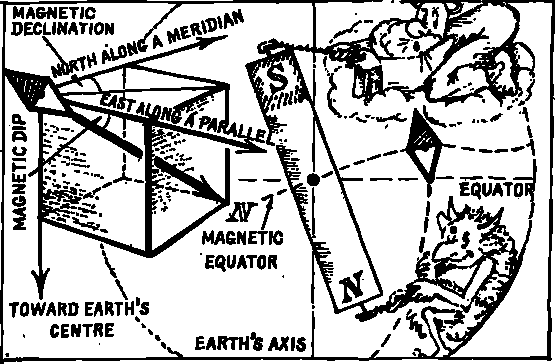
\includegraphics[width=\textwidth]{figures/fig-03-10.pdf}
\caption{The relative positions of Earth's axis and magnetic poles.}
\label{fig-3.10}
\end{figure}


From this moment, the study of geomagnetism was raised to a new level. More precise investigations showed that a magnetic needle does not point exactly north. The deviation of a compass needle from the meridian passing through the given point is called the magnetic declination. The magnetic pole's are displaced with respect to the earth's axis by \ang{11.5} (\figr{fig-3.10}). The needle is not exactly in a horizontal plane but points downward (in the northern hemisphere) through an angle, varying at various latitudes, called the magnetic dip. After measuring the magnetic dip at various points on the earth, we come to the conclusion that the magnetic ``dipole'' is deep within the earth. It sets up a nonuniform field, the non-uniformity reaching \SI{0.6d-4}{\tesla} at the magnetic poles and \SI{0.3d-4}{\tesla} at the equator.

What is this ``magnet'' inside the earth? The magnetic ``dipole'' is in the earth's core, which consists mainly of molten iron. Even in the molten state iron remains a good conductor of electricity. On this basis, a model constituting a sort of ``magnetic dynamo'' has been proposed to explain the earth's magnetic field. We shall not describe this model. It is sufficient to point out that the ``terrestrial magnet'' is the result of currents passing through the molten iron core.

The earth's magnetic field varies. The magnetic poles are continually being displaced at a rate of 5 or \SI{6}{\kilo\meter} per year. This is a negligible displacement on the scale of the whole earth and is a phenomenon that can be observed only in the course of hundreds of years. This is why it has been called the secular variation of the earth's magnetic field.

It is needless to demonstrate how vitally important it is to have an exact knowledge of all the elements of terrestrial magnetism at any point on our planet. The magnetic compass still serves navigators. This being the case, they must be furnished with maps showing the magnetic declinations and dips. Near the poles, as is shown in \figr{fig-3.10}, the north end of a magnetic needle no longer points toward the north. Near the equator, it is also difficult to manage without a magnetic map. The magnetic equator does not coincide at all with the line of zero latitude (true equator).

A precise knowledge of the earth's magnetic field is also of immense interest on land, as well, because it can be of service in geological surveys. But we cannot dwell on these problems. Geological physics, or geophysics, is a significant and extensive field of science and deserves a special discussion.

We shall devote a few words to so-called paleomagnetic investigations that give us an idea of the earth's magnetic field in ancient and prehistoric times. These investigations are based mainly on a study of remanent (residual) magnetization of rock, etc.

The following is the essence of methods employed for the prehistoric period. Bricks and clay pottery have a small remanent magnetism that is developed in the hot clay when it is being fired. The direction of the magnetic moment coincides with that of the magnetic field at the time the item was fired and cooled. Sometimes it is possible to determine the position of the item during its manufacture.

Another example of similar investigations is finding the geographic direction of the magnetic moment of an ore, its age being determined by the amounts of radioactive isotopes.

Paleomagnetic investigations are the most rigorous proof of continental drift. It was found that the magnetism of iron ore deposits, formed several hundreds of millions of years ago on the various continents, can be directed along the lines of force of the earth's magnetic field if the continents are brought together into a single vast continent Panganea which split into two supercontinents Laurasia and Gondwanaland. Later these continents were further split up, dividing Gondwanaland, for instance, into Africa, Australia, Antarctica and South America, which then gradually drifted apart.

So far we have mentioned only the intra-terrestrial origin of magnetism, and this is actually its main source. Certain changes occur, however, in the magnetic field of the earth due to charged particles arriving from space. These are chiefly streams of protons and electrons emitted by the sun. The charged particles are carried by the field to the magnetic poles and are rotated there in a circle by the Lorentz forces. This leads to two phenomena. In the first place, the moving charged particles set up a supplementary magnetic field consisting of magnetic storms. Secondly, they ionize the molecules of atmospheric gases, producing the aurora borealis, commonly called the northern lights (this is in the Northern Hemisphere: the lights seen in the Southern Hemisphere are called the aurora australis. Severe magnetic storms occur periodically (after 11.5 years). This period coincides with the periods of intensive solar activity.

Direct measurements by means of spacecraft indicate that the bodies nearest to the earth -- the moon, and the planets of Venus and Mars -- do not have their own magnetic field similar to that of the earth. Of the other planets of the solar system, only Jupiter and, evidently, Saturn have their own magnetic fields. A field of a strength up to \SI{10}{\gauss} and a number of typical phenomena (magnetic storms, synchrotron radio-frequency radiation, etc.) were discovered on Jupiter.

\section{Magnetic Fields of the Stars}

Magnetism is found, not only on planets and extinct stars, but on incandescent heavenly bodies as well. Since the sun is our nearest star, we know more about its magnetic field than that of other stars. The magnetic field of the sun can be visually observed during solar eclipses. Particles of solar material that have a magnetic moment align themselves along the lines of force, thereby sketching a picture of these lines. The magnetic poles are clearly seen and the strength of the magnetic field can be estimated. In regions of a size of the order of tens of thousands of kilometres, this field is of a strength a thousand times greater than that of the earth's field. These regions are called \emph{sunspots}. Since the spots are darker than the rest of the sun's surface, the temperature here must be lower, namely, 2000 degrees below the ``normal'' temperature of the sun.

Without doubt, the lower temperature and the stronger magnetic field are related in some way. But no proper theory relating these two facts has yet been proposed.

What about the other stars? The advances in astrophysics have been so amazing in recent years that it is now feasible to establish the existence of magnetic fields on the stars. It was found that these ``stellar magnetic spots'' have a temperature of about \SI{10000}{\celsius} and can change their position or even disappear entirely in the course of several months. It is simpler to explain these changes if we assume that the whole star rotates rather than have spots change their location.

The presence of magnetic fields is indicated by the anomalous intensity of certain spectral lines. It would seem that magnetic stars have an increased iron content on their magnetic equator.

Magnetic fields in space are very weak (a millionth of a gauss). This needs no explanation because an extremely high vacuum reigns in space. When stars are formed of atoms scattered throughout the universe, the condensing of the stellar material is accompanied by a ``condensing'' of the magnetic field. Why, then, do not all stars have a magnetic field?

The earth has existed for thousands of millions of years. It follows that the magnetic field of the earth is continually maintained by the electric currents flowing in its depths. Certain stars, having no magnetic field, have evidently cooled to an extent that they no longer have electric currents inside them. It is improbable, however, that this explanation is a universal one.
